% -*- latex -*-
%%%%%%%%%%%%%%%%%%%%%%%%%%%%%%%%%%%%%%%%%%%%%%%%%%%%%%%%%%%%%%%%
%%%%%%%%%%%%%%%%%%%%%%%%%%%%%%%%%%%%%%%%%%%%%%%%%%%%%%%%%%%%%%%%
%%%%
%%%% This text file is part of the source of 
%%%% `Introduction to High-Performance Scientific Computing'
%%%% by Victor Eijkhout, copyright 2012-6
%%%%
%%%% This book is distributed under a Creative Commons Attribution 3.0
%%%% Unported (CC BY 3.0) license and made possible by funding from
%%%% The Saylor Foundation \url{http://www.saylor.org}.
%%%%
%%%%
%%%%%%%%%%%%%%%%%%%%%%%%%%%%%%%%%%%%%%%%%%%%%%%%%%%%%%%%%%%%%%%%
%%%%%%%%%%%%%%%%%%%%%%%%%%%%%%%%%%%%%%%%%%%%%%%%%%%%%%%%%%%%%%%%

In this section we will look at how different ways of programming can
influence the performance of a code. This will only be an introduction
to the topic; for further discussion see the book by Goedeker and
Hoisie~\cite{Goedeker:performance-book}.

The full listings of the codes and explanations of the data graphed
here can be found in chapter~\ref{app:codes}. All performance results
were obtained on the \indextermbus{AMD}{Opteron} processors of the Ranger
computer~\cite{tacc:ranger}.

\Level 1 {Peak performance}

For marketing purposes, it may be desirable to define a `top speed' for a
CPU. Since a pipelined floating point unit can yield one result per
cycle asymptotically, you would calculate the theoretical
\indexterm{peak performance} as the product of the clock speed (in
ticks per second), number of floating point units, and the number of
cores; see section~\ref{sec:multicore}.  This top speed is
unobtainable in practice, and very few codes come even close to it.
The \indextermbus{Linpack}{benchmark} is one of the measures how close
you can get to it; the parallel version of this benchmark is reported
in the `top 500'; see section~\ref{sec:top500}. 

\Level 1 {Pipelining}
\label{sec:coding-pipeline}
\index{pipeline|(}

In section~\ref{sec:pipeline} you learned that the floating point
units in a modern CPU are pipelined, and that pipelines require a
number of independent operations to function efficiently. The typical
pipelineable operation is a vector addition; an example of an
operation that can not be pipelined is the inner product accumulation
\begin{verbatim}
for (i=0; i<N; i++)
  s += a[i]*b[i]
\end{verbatim}
The fact that \n{s} gets both read and written halts the addition
pipeline. One way to fill the \indexterm{floating point pipeline}
is to apply \indextermbusdef{loop}{unrolling}:
\begin{verbatim}
for (i = 0; i < N/2-1; i ++) {
  sum1 += a[2*i] * b[2*i];
  sum2 += a[2*i+1] * b[2*i+1];
}
\end{verbatim}
Now there are two independent multiplies in between the accumulations.
With a little indexing optimization this becomes:
\begin{verbatim}
for (i = 0; i < N/2-1; i ++) {
  sum1 += *(a + 0) * *(b + 0);
  sum2 += *(a + 1) * *(b + 1);

  a += 2; b += 2;
}
\end{verbatim}
A first observation about this code is that we are implicitly using
associativity and commutativity of addition: while the same quantities
are added, they are now in effect added in a different order. As you
will see in chapter~\ref{ch:arithmetic}, in computer arithmetic
this is not guaranteed to
give the exact same result. 

In a further optimization, we disentangle the addition and
multiplication part of each instruction. The hope is that while the
accumulation is waiting for the result of the multiplication, the
intervening instructions will keep the processor busy, in effect
increasing the number of operations per second.
\begin{verbatim}
for (i = 0; i < N/2-1; i ++) {
  temp1 = *(a + 0) * *(b + 0);
  temp2 = *(a + 1) * *(b + 1);

  sum1 += temp1; sum2 += temp2;

  a += 2; b += 2;
}
\end{verbatim}
Finally, we realize that the furthest we can move the addition away
from the multiplication, is to put it right in front of the
multiplication \emph{of the next iteration}:
\begin{verbatim}
for (i = 0; i < N/2-1; i ++) {
  sum1 += temp1;
  temp1 = *(a + 0) * *(b + 0);

  sum2 += temp2;
  temp2 = *(a + 1) * *(b + 1);

  a += 2; b += 2;
}
s = temp1 + temp2;
\end{verbatim}
Of course, we can unroll the operation by more than a factor of
two. While we expect an increased performance because of the longer
sequence of pipelined operations, large unroll factors
need large numbers of registers. Asking for more registers than a CPU
has is called \indextermbus{register}{spill}, and it will decrease
performance.

Another thing to keep in mind is that the total number of operations
is unlikely to be divisible by the unroll factor. This requires
\indexterm{cleanup code} after the loop to account for the final
iterations. Thus, unrolled code is harder to write than straight code,
and people have written tools to perform such
\indexterm{source-to-source transformations} automatically.

Cycle times for unrolling the inner product operation up to six times
are given in table~\ref{tab:unroll-inner}. Note that the timings do
not show a monotone behaviour at the unrolling by four. This sort of
variation is due to various memory-related factors.

\begin{table}[ht]
\leavevmode\kern\unitindent
  \begin{tabular}{|rrrrrr|}
    \hline
    1&2&3&4&5&6\\ \hline 6794&507&340&359&334&528\\ \hline
  \end{tabular}
  \caption{Cycle times for the inner product operation, unrolled up to
    six times}
  \label{tab:unroll-inner}
\end{table}

\index{pipeline|)}

\Level 1 {Cache size}
\label{sec:coding-cachesize}

Above, you learned that data from L1 can be moved with lower latency
and higher bandwidth than from~L2, and L2 is again faster than L3 or
memory. This is easy to demonstrate with code that repeatedly access
the same data:
\begin{verbatim}
for (i=0; i<NRUNS; i++)
  for (j=0; j<size; j++)
    array[j] = 2.3*array[j]+1.2;
\end{verbatim}
If the size parameter allows the array to fit in cache, the operation
will be relatively fast. As the size of the dataset grows, parts of it
will evict other parts from the L1 cache, so the speed of the
operation will be determined by the latency and bandwidth of the L2
cache. This can be seen in figure~\ref{fig:cache-overflow}.
\begin{figure}[ht]
  \begin{quote}
  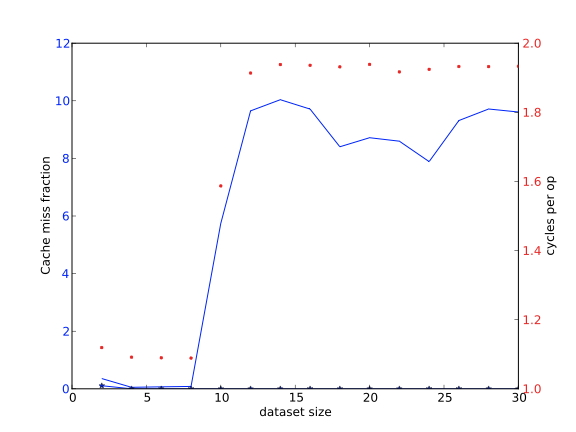
\includegraphics[scale=.5]{graphics/cacheoverflow}
  \end{quote}
  \caption{Average cycle count per operation as function of the
    dataset size}
  \label{fig:cache-overflow}
\end{figure}
The full code is given in section~\ref{sec:cachesize-code}.

\begin{exercise}
  Argue that with a large enough problem and an \ac{LRU} replacement policy
  (section~\ref{sec:lru}) essentially all data in the L1 will be
  replaced in every iteration of the outer loop. Can you write an
  example code that will let some of the L1 data stay resident?
\end{exercise}

Often, it is possible to arrange the operations to keep data in L1
cache. For instance, in our example, we could write
\begin{verbatim}
for (b=0; b<size/l1size; b++) {
  blockstart = 0;
  for (i=0; i<NRUNS; i++) {
    for (j=0; j<l1size; j++)
      array[blockstart+j] = 2.3*array[blockstart+j]+1.2; 
  }
  blockstart += l1size;
}
\end{verbatim}
assuming that the L1 size divides evenly in the dataset size.
This strategy is called \indextermbus{cache}{blocking} or
\indexterm{blocking for cache reuse}.

\begin{exercise}
  To arrive at the blocked code, the loop over \n{j} was split into a
  loop over blocks and an inner loop over the elements of the block;
  the outer loop over \n{i} was then exchanged with the loop over the
  blocks. In this particular example you could also simply exchange
  the \n{i} and \n{j} loops. Why may this not be optimal for performance?
\end{exercise}

\Level 1 {Cache lines}
\label{sec:coding-cacheline}

Since data is moved from memory to cache in consecutive chunks named
cachelines (see section~\ref{sec:cacheline}), code that does not
utilize all data in a cacheline pays a bandwidth penalty. This is born
out by a simple code
\begin{verbatim}
for (i=0,n=0; i<L1WORDS; i++,n+=stride)
  array[n] = 2.3*array[n]+1.2;
\end{verbatim}
Here, a fixed number of operations is performed, but on elements that
are at distance \n{stride}. As this \indexterm{stride} increases, we expect an
increasing runtime, which is born out by
\begin{figure}[ht]
  \begin{quote}
  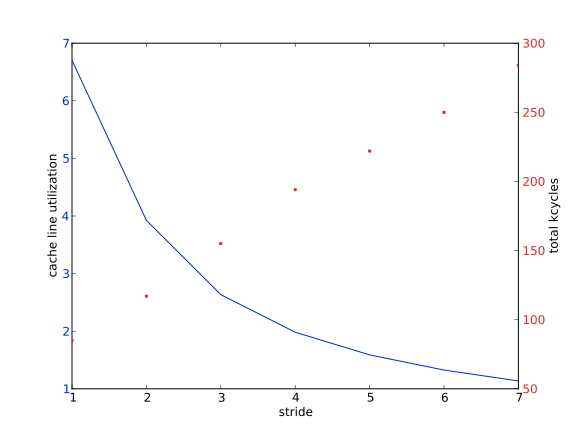
\includegraphics[scale=.5]{graphics/cacheline8}
  \end{quote}
  \caption{Run time in kcycles and L1 reuse as a function of stride}
  \label{fig:cacheline}
\end{figure}
the graph in figure~\ref{fig:cacheline}.

The graph also shows a decreasing reuse of cachelines, defined as the
number of vector elements divided by the number of L1 misses (on
stall; see section~\ref{sec:prefetch}). 

The full code is given in section~\ref{sec:cacheline-code}.

\Level 1 {TLB}
\label{sec:coding-tlb}

As explained in section~\ref{sec:tlb}, the \acf{TLB} maintains a small
list of frequently used memory pages and their locations; addressing
data that are location on one of these pages is much faster than data
that are not. Consequently, one wants to code in such a way that the
number of pages accessed is kept low.

Consider code for traversing the elements of a two-dimensional array
in two different ways.
\begin{verbatim}
#define INDEX(i,j,m,n) i+j*m
array = (double*) malloc(m*n*sizeof(double));

/* traversal #1 */
for (j=0; j<n; j++)
  for (i=0; i<m; i++)
    array[INDEX(i,j,m,n)] = array[INDEX(i,j,m,n)]+1;

/* traversal #2 */
for (i=0; i<m; i++)
  for (j=0; j<n; j++)
    array[INDEX(i,j,m,n)] = array[INDEX(i,j,m,n)]+1;
\end{verbatim}

The results (see Appendix~\ref{sec:tlb-code} for the source code) are
plotted in figures \ref{fig:tlb_row} and~\ref{fig:tlb_col}. 

\begin{figure}[ht]
  \begin{quote}
  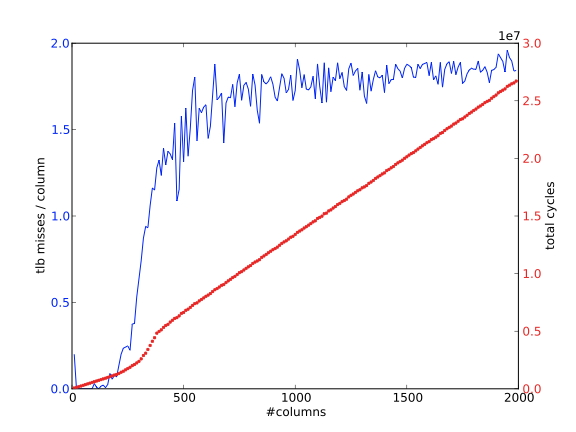
\includegraphics[scale=.5]{graphics/tlb_col}
  \end{quote}
  \caption{Number of TLB misses per column as function of the number
    of columns; columnwise traversal of the array.}
  \label{fig:tlb_col}
\end{figure}
\begin{figure}[ht]
  \begin{quote}
  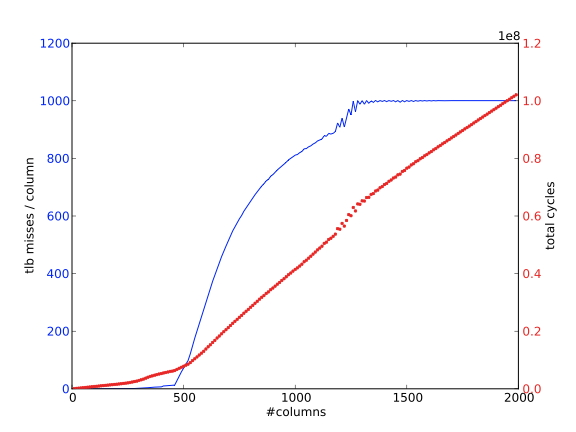
\includegraphics[scale=.5]{graphics/tlb_row}
  \end{quote}
  \caption{Number of TLB misses per column as function of the number
    of columns; rowwise traversal of the array.}
  \label{fig:tlb_row}
\end{figure}

Using $m=1000$ means that, on the \indextermbus{AMD}{Opteron} which
has pages of $512$ doubles, we need roughly two pages for each
column. We run this example, plotting the number `TLB misses', that
is, the number of times a page is referenced that is not recorded in
the TLB.
\begin{enumerate}
\item In the first traversal this is indeed what happens. After we
  touch an element, and the TLB records the page it is on, all other
  elements on that page are used subsequently, so no further TLB
  misses occur. Figure~\ref{fig:tlb_col} shows that, with increasing~$n$,
  the number of TLB misses per column is roughly two.
\item In the second traversal, we touch a new page for every element
  of the first row. Elements of the second row will be on these pages,
  so, as long as the number of columns is less than the number of TLB
  entries, these pages will still be recorded in the TLB. As the
  number of columns grows, the number of TLB increases, and ultimately
  there will be one TLB miss for each element
  access. Figure~\ref{fig:tlb_row} shows that, with a large enough number
  of columns, the number of TLB misses per column is equal to the
  number of elements per column.
\end{enumerate}

\Level 1 {Cache associativity}
\label{sec:assoc-coding}

There are many algorithms that work by recursive division of a
problem, for instance the \indexac{FFT} algorithm. As a result, code
for such algorithms will often operate on vectors whose length is a power of
two. Unfortunately, this can cause conflicts with certain
architectural features of a CPU, many of which involve powers of two.

In section~\ref{sec:directmap} you saw how
the operation of adding a small number of vectors
\[ \forall_j\colon y_j= y_j+\sum_{i=1}^mx_{i,j} \]
is a problem for direct mapped caches or set-associative caches with
associativity.

As an example we take the
\indextermbus{AMD}{Opteron}, which has an L1 cache of 64K bytes, and
which is two-way set associative. Because of the set associativity,
the cache can handle two addresses being mapped to the same cache
location, but not three or more. Thus, we let the vectors be of
size~$n=4096$ doubles, and we measure the effect in cache misses and
cycles of letting $m=1,2,\ldots$.

\begin{figure}
  \begin{quote}
  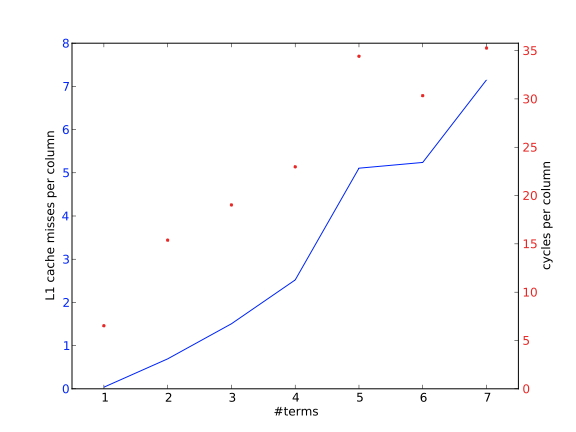
\includegraphics[scale=.5]{graphics/l1_assoc}
  \end{quote}
  \caption{The number of L1 cache misses and the number of cycles for
    each $j$ column accumulation, vector length~$4096$}
  \label{fig:l1_assoc}
\end{figure}

\begin{figure}
  \begin{quote}
  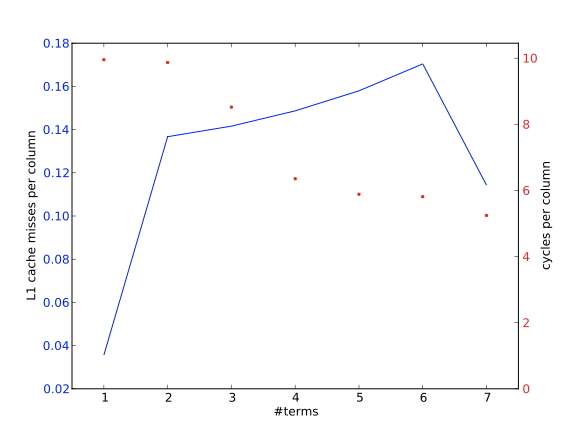
\includegraphics[scale=.5]{graphics/l1_assocshift}
  \end{quote}
  \caption{The number of L1 cache misses and the number of cycles for
    each $j$ column accumulation, vector length~$4096+8$}
  \label{fig:l1_assoc_shift}
\end{figure}

First of all, we note that we use the vectors sequentially, so, with a
cacheline of eight doubles, we should ideally see a cache miss rate of
$1/8$ times the number of vectors~$m$. Instead, in
figure~\ref{fig:l1_assoc} we see a rate approximately proportional
to~$m$, meaning that indeed cache lines are evicted immediately. The
exception here is the case $m=1$, where the two-way associativity
allows the cachelines of two vectors to stay in cache.

Compare this to figure~\ref{fig:l1_assoc_shift}, where we used a
slightly longer vector length, so that locations with the same $j$ are
no longer mapped to the same cache location. As a result, we see a
cache miss rate around $1/8$, and a smaller number of cycles,
corresponding to a complete reuse of the cache lines. 

Two remarks: the cache miss numbers are in fact lower than the theory
predicts, since the processor will use prefetch streams. Secondly, in
figure~\ref{fig:l1_assoc_shift} we see a decreasing time with
increasing~$m$; this is probably due to a progressively more
favourable balance between load and store operations. Store operations
are more expensive than loads, for various reasons.

\Level 1 {Loop nests}
\index{loop!nested|(}

If your code has \emph{nested loops}, and the iterations of the outer
loop are independent, you have a choice which loop to make outer and
which to make inner.

\begin{exercise}
  Give an example of a doubly-nested loop where the loops can be
  exchanged; give an example where this can not be done. If at all
  possible, use practical examples from this book.
\end{exercise}

If you have such choice, there are many factors that can influence
your decision.

\heading{Programming language: C~versus~Fortran}
%
If your loop describes the $(i,j)$ indices of a two-dimensional array,
it is often best to let the $i$-index be in the inner loop for
Fortran, and the $j$-index inner for~C.

\begin{exercise}
  Can you come up with at least two reasons why this is possibly better for performance?
\end{exercise}

However, this is not a hard-and-fast rule. It can depend on the size
of the loops, and other factors. For instance, in the matrix-vector
product, changing the loop ordering changes how the input and output
vectors are used.

\heading{Parallelism model}
%
If you want to parallelize your loops with \indexterm{OpenMP}, you
generally want the outer loop to be larger than the inner. Having a
very short outer loop is definitely bad. A~short inner loop can also
often be \emph{vectorized by the
  compiler}\index{compiler!vectorization}.

On the other hand, if you are targeting a \indexac{GPU}, you want the
large loop to be the inner one. The unit of parallel work should not have branches
or loops.

\index{loop!nested|)}

\Level 1 {Loop tiling}
\label{sec:loop-tiling}

In some cases performance can be increased by breaking up a loop into
two nested loops, an outer one for the blocks in the iteration space,
and an inner one that goes through the block. This is known as
\indextermbusdef{loop}{tiling}: the (short) inner loop is a tile, many
consecutive instances of which form the iteration space.

For instance
\begin{verbatim}
for (i=0; i<n; i++)
  ...
\end{verbatim}
becomes
\begin{verbatim}
bs = ...       /* the blocksize */
nblocks = n/bs /* assume that n is a multiple of bs */
for (b=0; b<nblocks; b++)
  for (i=b*bs,j=0; j<bs; i++,j++)
    ...
\end{verbatim}
For a single loop this may not make any difference, but given the
right context it may. For instance, if an array is repeatedly used,
but it is too large to fit into cache:
\begin{verbatim}
for (n=0; n<10; n++)
  for (i=0; i<100000; i++)
    ... = ...x[i] ...

\end{verbatim}
then loop tiling may lead to a situation where the array is divided
into blocks that will fit in cache:
\begin{verbatim}
bs = ... /* the blocksize */
for (b=0; b<100000/bs; b++)
  for (n=0; n<10; n++)
    for (i=b*bs; i<(b+1)*bs; i++)
      ... = ...x[i] ...
\end{verbatim}
For this reason, loop tiling is also known as
\indextermbus{cache}{blocking}. The block size depends on how much
data is accessed in the loop body; ideally you would try to make data
reused in L1 cache, but it is also possible to block for L2 reuse. Of
course, L2 reuse will not give as high a performance as L1 reuse.

\begin{exercise}
  Analyze this example. When is \n{x} brought into cache, when is it
  reused, and when is it flushed? What is the required cache size in
  this example? Rewrite this example, using a constant
\begin{verbatim}
#define L1SIZE 65536
\end{verbatim}
\end{exercise}

For a less trivial example, let's look at
\indextermbus{matrix}{transposition} $A\leftarrow B^t$. Ordinarily you would traverse
the input and output matrices:
%
\verbatimsnippet{regulartranspose}
%
Using blocking this becomes:
%
\verbatimsnippet{blockedtranspose}
%
Unlike in the example above, each element of the input and output is
touched only once, so there is no direct reuse. However, there is
reuse of cachelines. 

\begin{figure}[ht]
  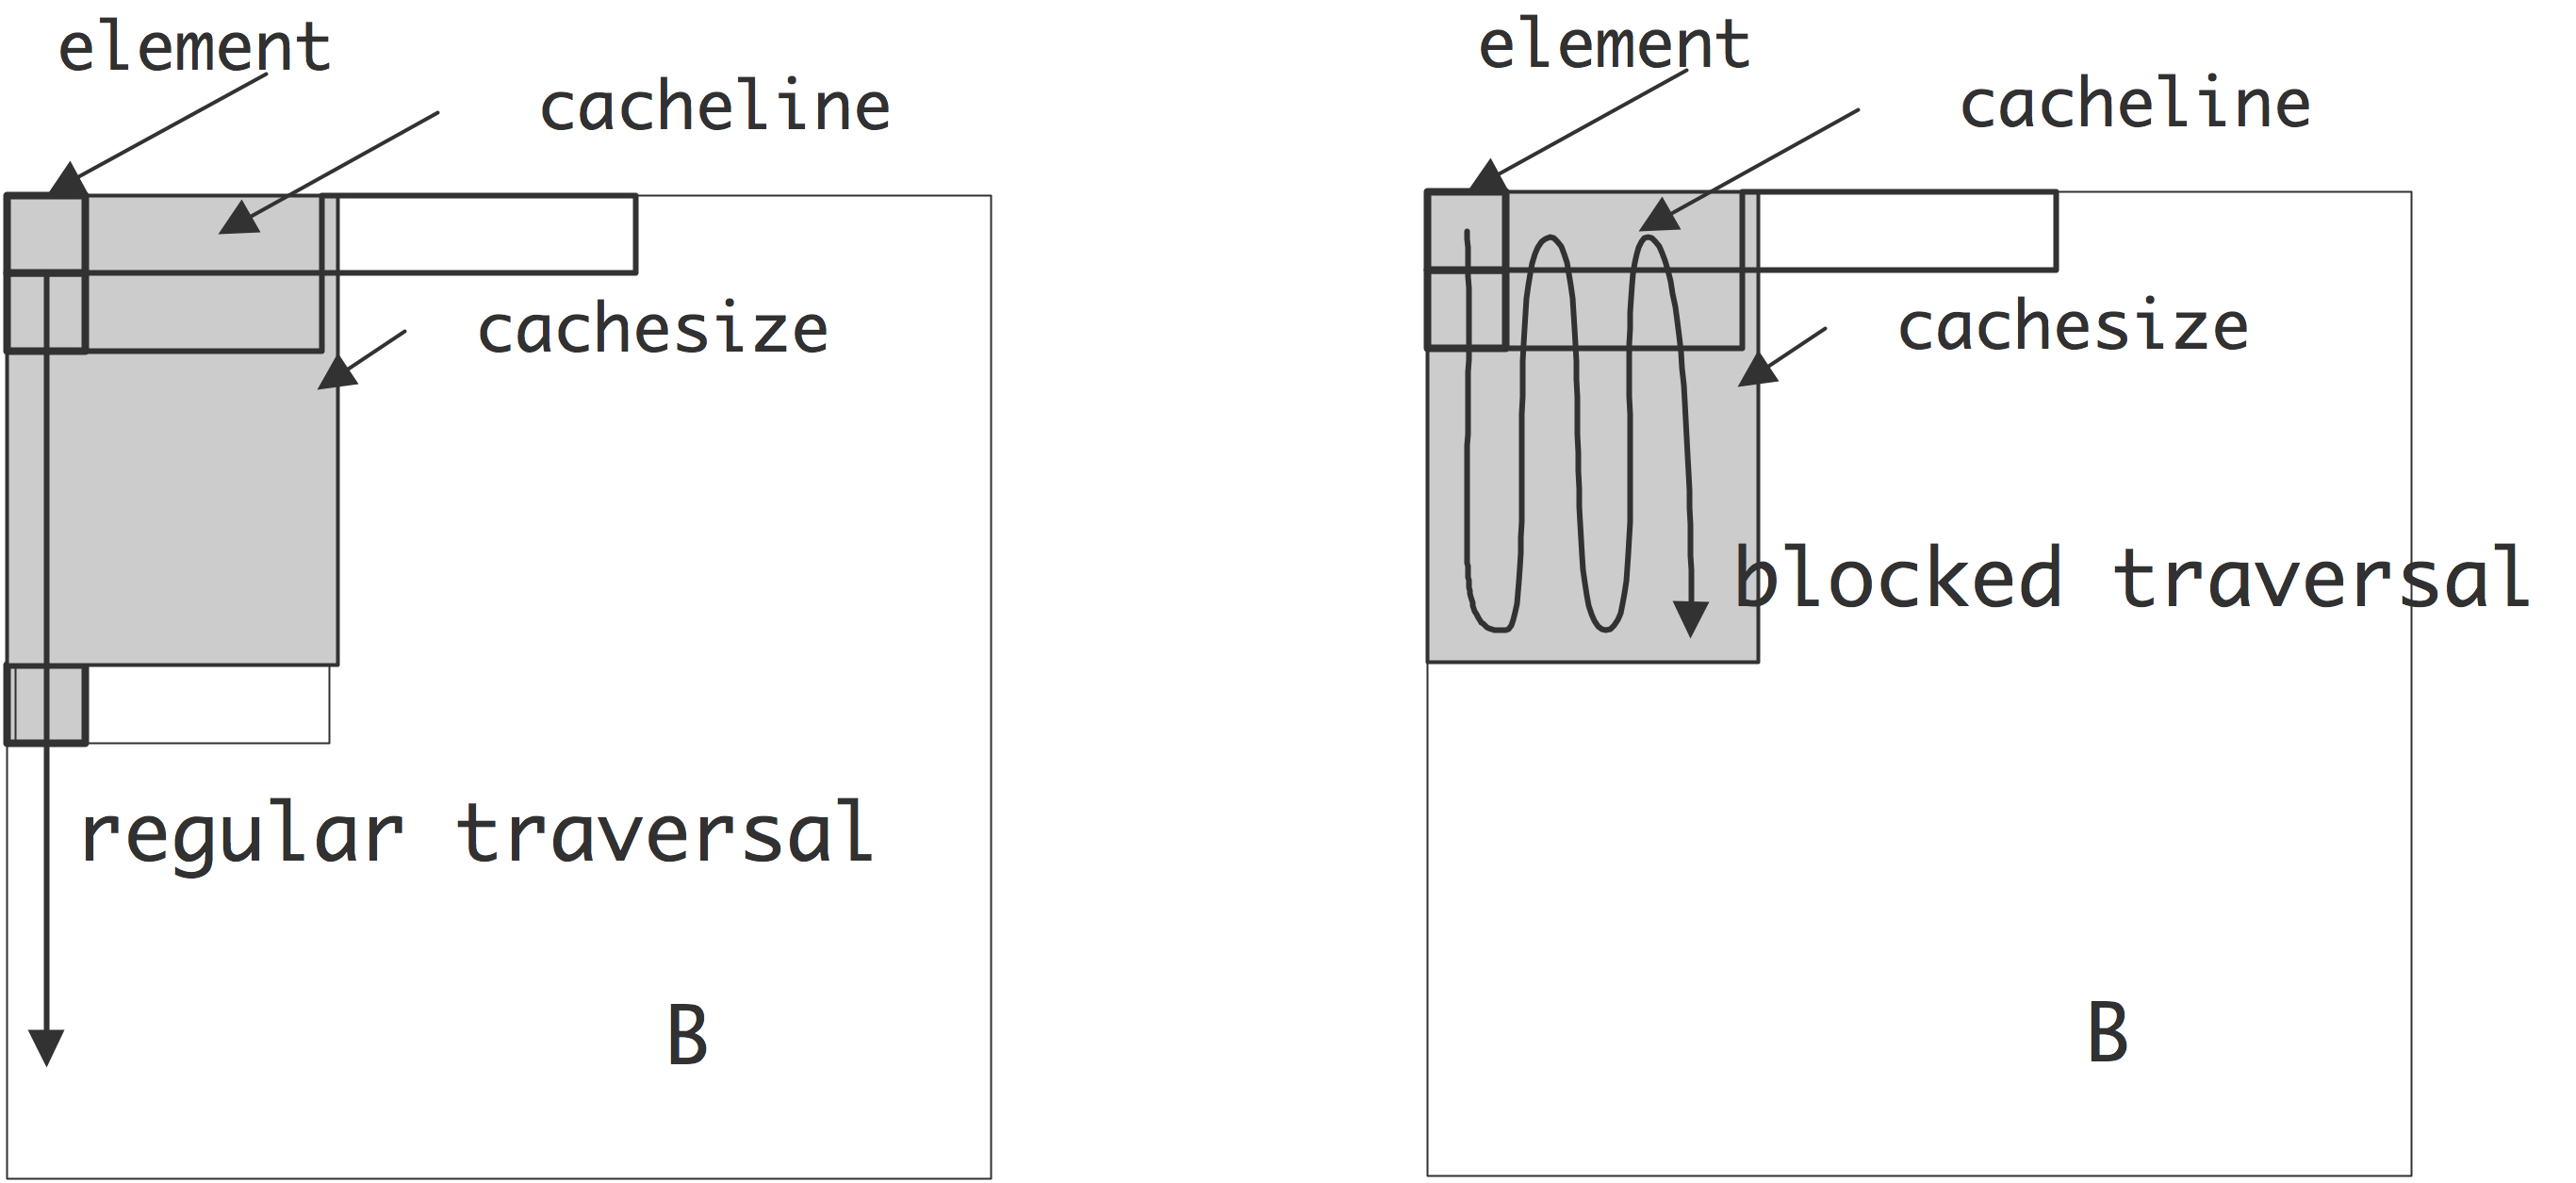
\includegraphics[scale=.13]{blockedtranspose}
  \caption{Regular and blocked traversal of a matrix}
  \label{fig:blockedtranspose}
\end{figure}
Figure~\ref{fig:blockedtranspose} shows how one of the matrices is
traversed in a different order from its storage order, for instance
columnwise while it is stored by rows. This has the effect that each
element load transfers a cacheline, of which only one element is
immediately used. In the regular traversal, this streams of cachelines
quickly overflows the cache, and there is no reuse. In the blocked
traversal, however, only a small number of cachelines is traversed
before the next element of these lines is needed. Thus there is reuse
of cachelines, or \indextermsub{spatial}{locality}.

The most important example of attaining performance through blocking
is the \indexterm{matrix-matrix product}.
In section~\ref{sec:locality} we looked at the matrix-matrix
multiplication, and concluded that little data could be kept in
cache. With loop tiling we can improve this situation. For instance,
the standard way of writing this product
\begin{verbatim}
for i=1..n
  for j=1..n
    for k=1..n
      c[i,j] += a[i,k]*b[k,j]
\end{verbatim}
can only be optimized to keep \n{c[i,j]} in register:
\begin{verbatim}
for i=1..n
  for j=1..n
    s = 0
    for k=1..n
      s += a[i,k]*b[k,j]
    c[i,j] += s
\end{verbatim}
Using loop tiling we can easily keep parts of~\n{a[i,:]} in cache,
assuming that \n{a} is stored by rows:
\begin{verbatim}
for kk=1..n/bs
  for i=1..n
    for j=1..n
      s = 0
      for k=(kk-1)*bs+1..kk*bs
        s += a[i,k]*b[k,j]
      c[i,j] += s
\end{verbatim}


\Level 1 {Optimization strategies}
\label{sec:scalar-opt}

\begin{figure}[ht]
  \begin{quote}
  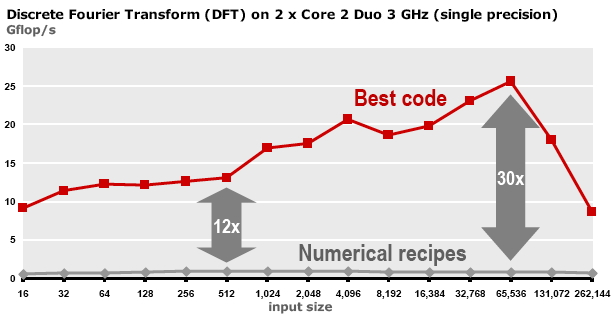
\includegraphics[scale=.5]{graphics/dft}
  \end{quote}
  \caption{Performance of naive and optimized implementations of the Discrete Fourier Transform}
  \label{fig:dft-perf}
\end{figure}

\begin{figure}[ht]
  \begin{quote}
  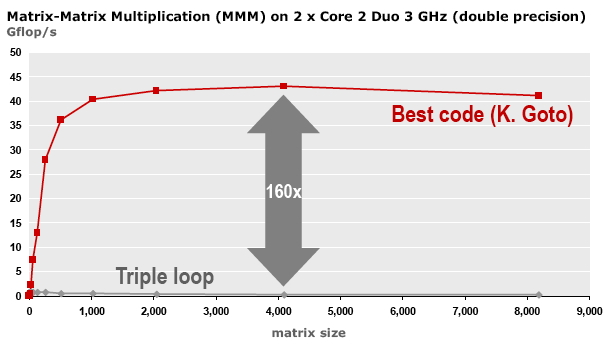
\includegraphics[scale=.5]{graphics/gemm}
  \end{quote}
  \caption{Performance of naive and optimized implementations of the matrix-matrix product}
  \label{fig:gemm-perf}
\end{figure}

Figures \ref{fig:dft-perf} and \ref{fig:gemm-perf} show that there can
be wide discrepancy between the performance of naive implementations
of an operation (sometimes called the `reference implementation'), and
optimized implementations. Unfortunately, optimized implementations
are not simple to find. For one, since they rely on blocking, their
loop nests are double the normal depth: the matrix-matrix
multiplication becomes a six-deep loop. Then, the optimal block size
is dependent on factors like the target architecture.

We make the following observations:
\begin{itemize}
\item Compilers\index{compiler} are not able to extract anywhere close
  to optimal performance\footnote{Presenting a compiler with the
    reference implementation may still lead to high performance, since
    some compilers are trained to recognize this operation. They will
    then forego translation and simply replace it by an optimized
    variant.}.
\item There are \indexterm{autotuning} projects for automatic
  generation of implementations that are tuned to the
  architecture. This approach can be moderately to very
  successful. Some of the best known of these projects are
  Atlas~\cite{atlas-parcomp} for Blas kernels, and
  Spiral~\cite{spiral} for transforms.
\end{itemize}

\Level 1 {Cache aware and cache oblivious programming}

Unlike registers and main memory, both of
which can be addressed in (assembly) code, use of caches is
implicit. There is no way a programmer can load data explicitly to a
certain cache, even in assembly language. 

However, it is possible to code in a `cache aware' manner. Suppose a
piece of code repeatedly operates on an amount of data that is less
than the cache size. We can assume that the first time the data is
accessed, it is brought into cache; the next time it is accessed it
will already be in cache. On the other hand, if the amount of data is
more than the cache size\footnote{We are conveniently ignoring matters
  of set-associativity here, and basically assuming a fully
  associative cache.}, it will partly or fully be flushed out of cache
in the process of accessing it.

We can experimentally demonstrate this phenomenon. With a very
accurate counter, the code fragment
\begin{verbatim}
for (x=0; x<NX; x++)
  for (i=0; i<N; i++)
    a[i] = sqrt(a[i]);
\end{verbatim}
will take time linear in \texttt{N} up to the point where \texttt{a}
fills the cache. An easier way to picture this is to compute a
normalized time, essentially a time per execution of the inner loop:
\begin{verbatim}
t = time();
for (x=0; x<NX; x++)
  for (i=0; i<N; i++)
    a[i] = sqrt(a[i]);
t = time()-t;
t_normalized = t/(N*NX);
\end{verbatim}
The normalized time will be constant until the array \texttt{a} fills
the cache, then increase and eventually level off again. (See
section~\ref{sec:coding-cachesize} for an elaborate discussion.)

The explanation is that,
as long as \texttt{a[0]...a[N-1]} fit in L1 cache, the inner loop will
use data from the L1 cache. Speed of access is then determined by the
latency and bandwidth of the L1 cache.
As the amount of data grows beyond the L1 cache size, some or all of
the data will be flushed from the L1, and performance will be determined by
the characteristics of the L2 cache. Letting the amount of data grow
even further, performance will again drop to a linear behaviour
determined by the bandwidth from main memory.

\index{cache!oblivious programming|(}

If you know the cache size, it is possible in cases such as above to
arrange the algorithm to use the cache optimally. However, the cache
size is different per processor, so this makes your code not portable,
or at least its high performance is not portable. Also, blocking for
multiple levels of cache is complicated. For these reasons, some
people advocate \emph{cache oblivious
  programming}~\cite{Frigo:oblivious}. 

Cache oblivious programming can be described as a way of programming
that automatically uses all levels of the
\indextermbus{cache}{hierarchy}. This is typically done by using a
\indexterm{divide-and-conquer} strategy, that is, recursive
subdivision of a problem.

As a simple example of cache oblivious programming is the \indextermbus{matrix}
{transposition} operation $B\leftarrow A^t$. First we observe that each
element of either matrix is accessed once, so the only reuse is in the
utilization of cache lines. If both matrices are stored by
rows and we traverse $B$ by rows, then $A$~is traversed by columns,
and for each element accessed one cacheline is loaded. If the number
of rows times the number of elements per cacheline is more than the
cachesize, lines will be evicted before they can be reused.

\begin{figure}[ht]
  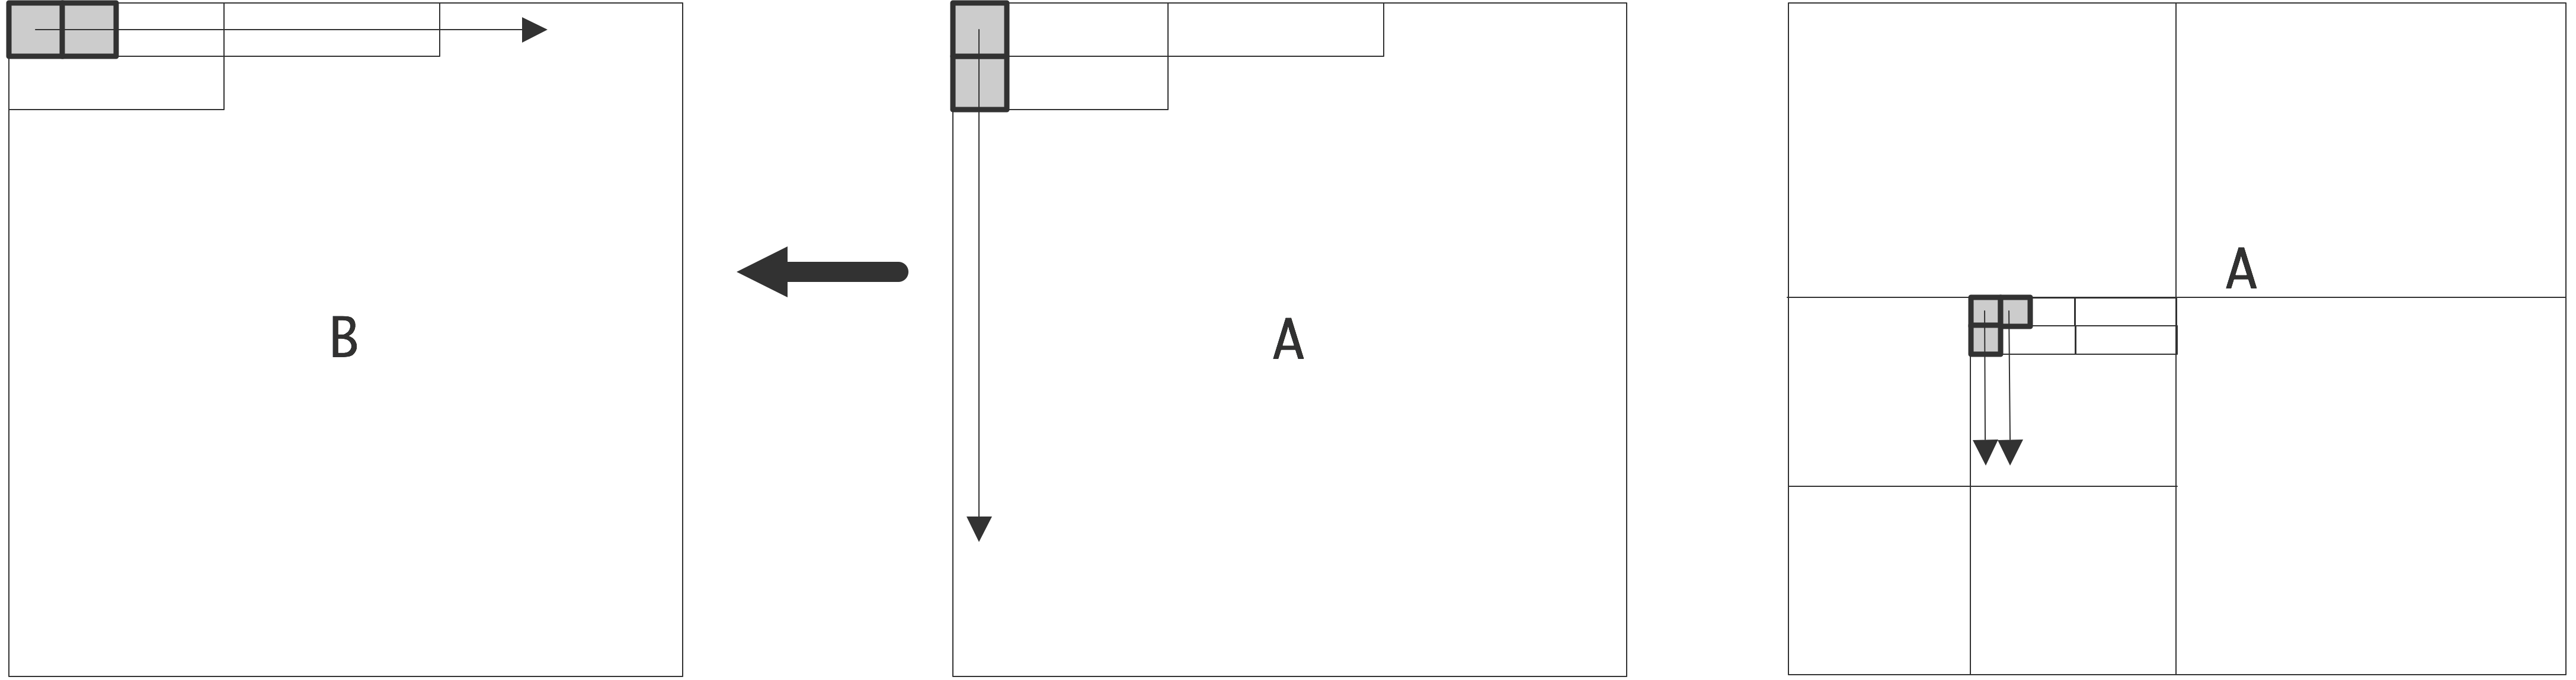
\includegraphics[scale=.1]{graphics/oblivious1}
  \caption{Matrix transpose operation, with simple and recursive
    traversal of the source matrix}
  \label{fig:oblivious-transpose}
\end{figure}
In a cache oblivious implementation we divide $A$ and~$B$ as
$2\times2$ block matrices, and recursively compute $B_{11}\leftarrow
A_{11}^t$, $B_{12}\leftarrow A_{21}^t$, et cetera; see
figure~\ref{fig:oblivious-transpose}. At some point in the recursion,
blocks $A_{ij}$ will now be small enough that they fit in cache, and
the cachelines of~$A$ will be fully used. Hence, this algorithm
improves on the simple one by a factor equal to the cacheline size.

The cache oblivious strategy can often yield improvement, but it is
not necessarily optimal. In the matrix-matrix product it improves on
the naive algorithm, but it is not as good as an algorithm that is
explicitly designed to make optimal use of
caches~\cite{GotoGeijn:2008:Anatomy}.

\index{cache!oblivious programming|)}

\Level 1 {Case study: Matrix-vector product}
\label{sec:mvp-opt}

Let us consider in some detail
the \indexterm{matrix-vector product}
\[ \forall_{i,j}\colon y_i\leftarrow a_{ij}\cdot x_j \] This involves $2n^2$
operations on $n^2+2n$ data items, so reuse is~$O(1)$: memory accesses
and operations are of the same order. However, we note that there is a
double loop involved, and the $x,y$ vectors have only a single index,
so each element in them is used multiple times.

Exploiting this theoretical reuse is not trivial. In
\begin{verbatim}
/* variant 1 */
for (i)
  for (j)
    y[i] = y[i] + a[i][j] * x[j];
\end{verbatim}
the element \texttt{y[i]} seems to be reused. However, the statement
as given here would write \texttt{y[i]} to memory in every inner
iteration, and we have to write the loop as
\begin{verbatim}
/* variant 2 */
for (i) {
  s = 0;
  for (j)
    s = s + a[i][j] * x[j];
  y[i] = s;
}
\end{verbatim}
to ensure reuse. This variant uses $2n^2$ loads and $n$~stores.

This code fragment only exploits the reuse
of~\texttt{y} explicitly. If the cache is too small to hold the whole
vector~\texttt{x} plus a column of~\texttt{a}, each element
of~\texttt{x} is still repeatedly loaded in every outer iteration.

Reversing the loops as
\begin{verbatim}
/* variant 3 */
for (j)
  for (i)
    y[i] = y[i] + a[i][j] * x[j];
\end{verbatim}
exposes the reuse of~\texttt{x}, especially if we write this as
\begin{verbatim}
/* variant 3 */
for (j) {
  t = x[j];
  for (i)
    y[i] = y[i] + a[i][j] * t;
}
\end{verbatim}
but now \texttt{y} is no longer
reused. Moreover, we now have $2n^2+n$ loads, comparable to variant~2,
but $n^2$~stores, which is of a higher order.

It is possible to get reuse both of $x$ and~$y$, but this requires
more sophisticated programming. The key here is to split the loops into
blocks. For instance:
\begin{verbatim}
for (i=0; i<M; i+=2) {
  s1 = s2 = 0;
  for (j) {
    s1 = s1 + a[i][j] * x[j];
    s2 = s2 + a[i+1][j] * x[j];
  }
  y[i] = s1; y[i+1] = s2;
}
\end{verbatim}
This is also called \indexterm{loop}{unrolling},
or \indexterm{strip mining}. The amount by which you unroll
loops is determined by the number of available registers.

\Level 1 {Case study: Goto matrix-matrix product}
\label{sec:goto-gemm}
\index{matrix-matrix product!Goto implementation|(textbf}

In section~\ref{sec:gemm} we already argued that the \indexterm{matrix-matrix
product} (or \indextermtt{dgemm} in Blas terms) has a large amount of
possible data reuse: there are $O(n^3)$ operations on $O(n^2)$ data.
We will now consider an implementation, due
to \indextermsub{Kazushige}{Goto}~\cite{GotoGeijn:2008:Anatomy}, that
indeed achieves close to peak performance.

The matrix-matrix algorithm has three loops, each of which we can block,
giving a six-way nested loop.
Since there are no recurrences on the output elements, all resulting
loop exchanges are legal. Combine this with the fact that the loop blocking
introduces three blocking parameters, and you'll see that the number of
potential implementations is enormous. Here we present the global reasoning
that underlies the Goto implementation; for a detailed discussion see the paper cited.

We start by writing the product $C\leftarrow A\cdot B$ (or
  $C\leftarrow C+AB$ according to the Blas standard) as a sequence of
  low-rank updates:
\[ C_{**} = \sum_k  A_{*k}B_{k*} \]
\begin{figure}[ht]
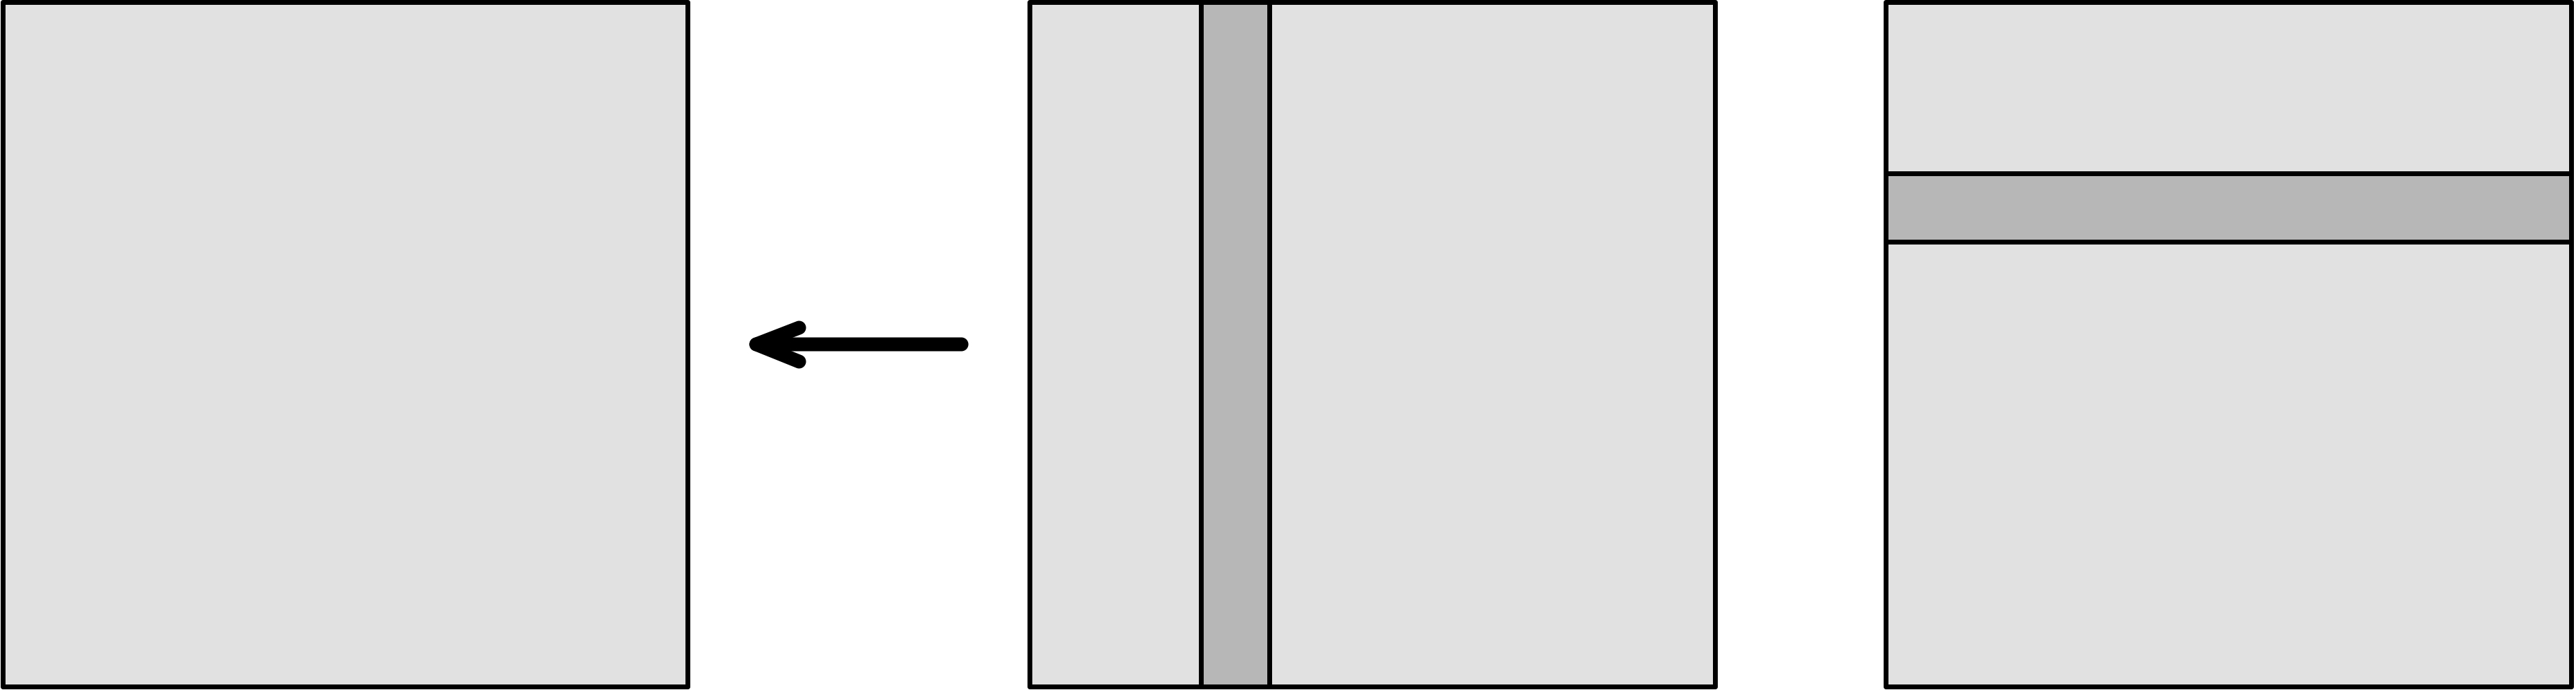
\includegraphics[scale=.1]{gotoblas1}
\caption{Matrix-matrix multiplication as a sequence of low-rank updates}
\label{fig:goto1}
\end{figure}
See figure~\ref{fig:goto1}. Next we derive the `block-panel' multiplication
by multiplying a block of~$A$ by a `sliver' of~$B$; see figure~\ref{fig:goto2}.
\begin{figure}[ht]
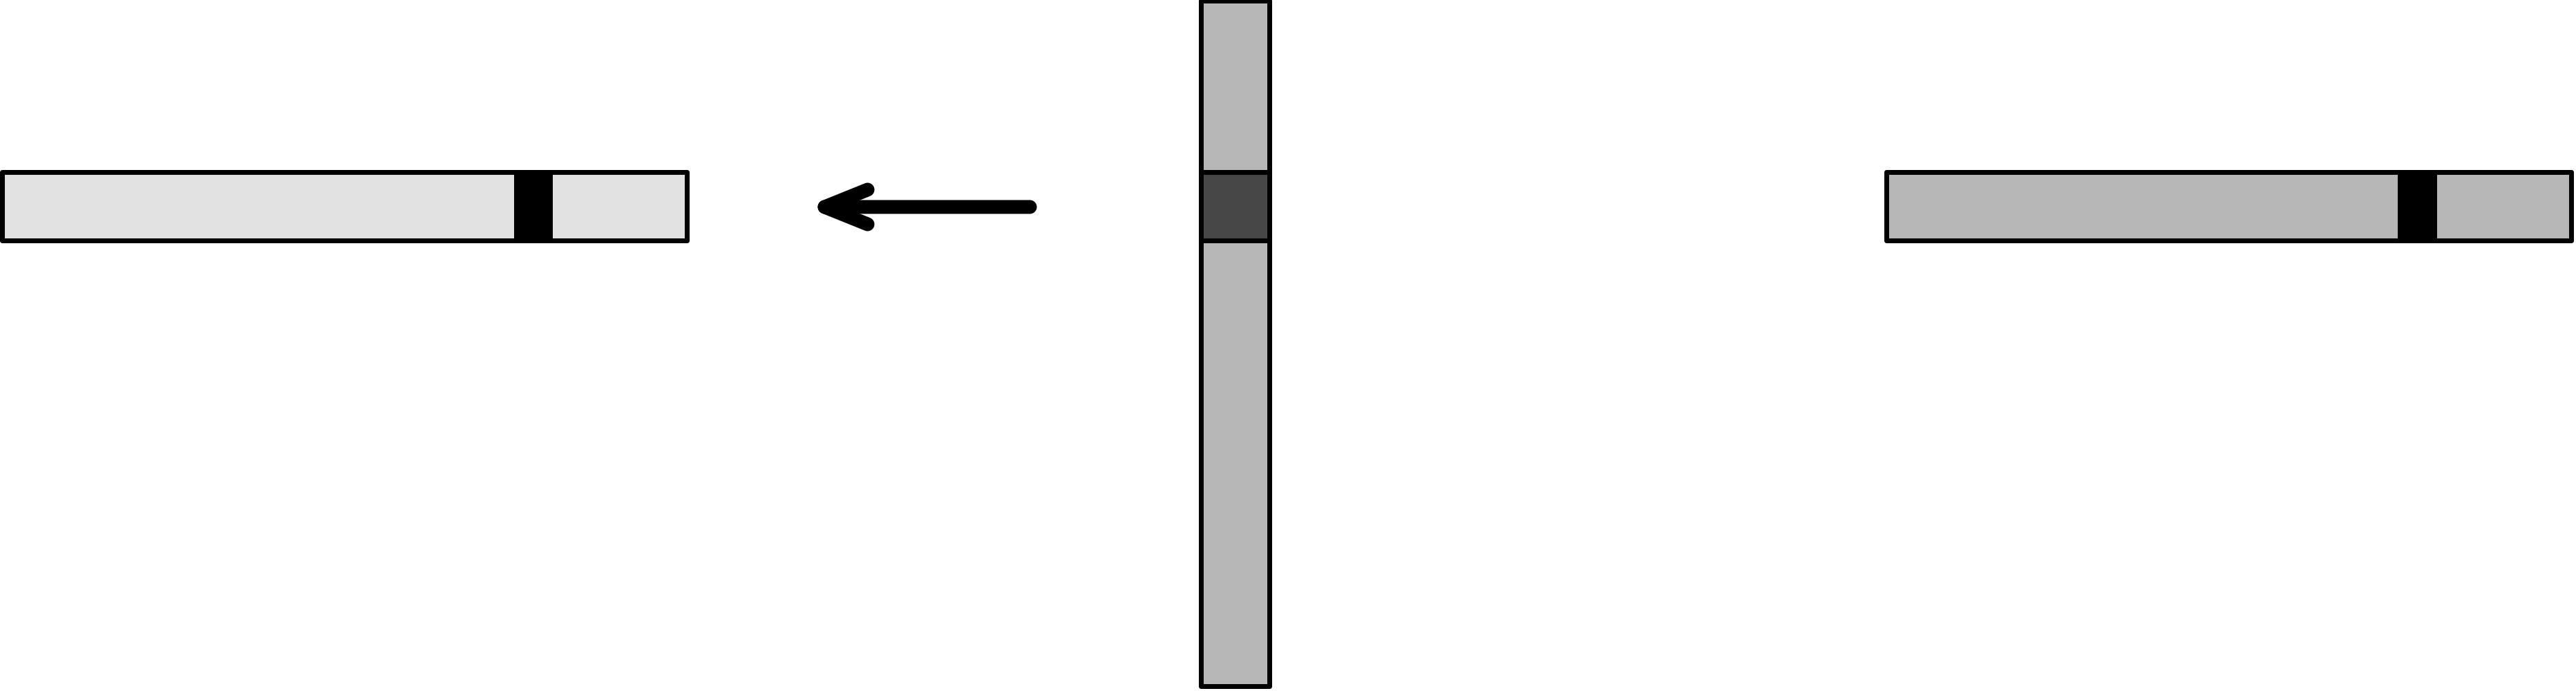
\includegraphics[scale=.1]{gotoblas2}  
\caption{The block-panel multiplication in the matrix-matrix algorithm}
\label{fig:goto2}
\end{figure}
Finally, the inner algorithm accumulates a small row $C_{i,*}$,
typically of small size such as~4, by accumulating:
\begin{verbatim}
// compute C[i,*] :
for k:
   C[i,*] = A[i,k] * B[k,*]
\end{verbatim}
See figure~\ref{fig:goto3}.
\begin{figure}[ht]
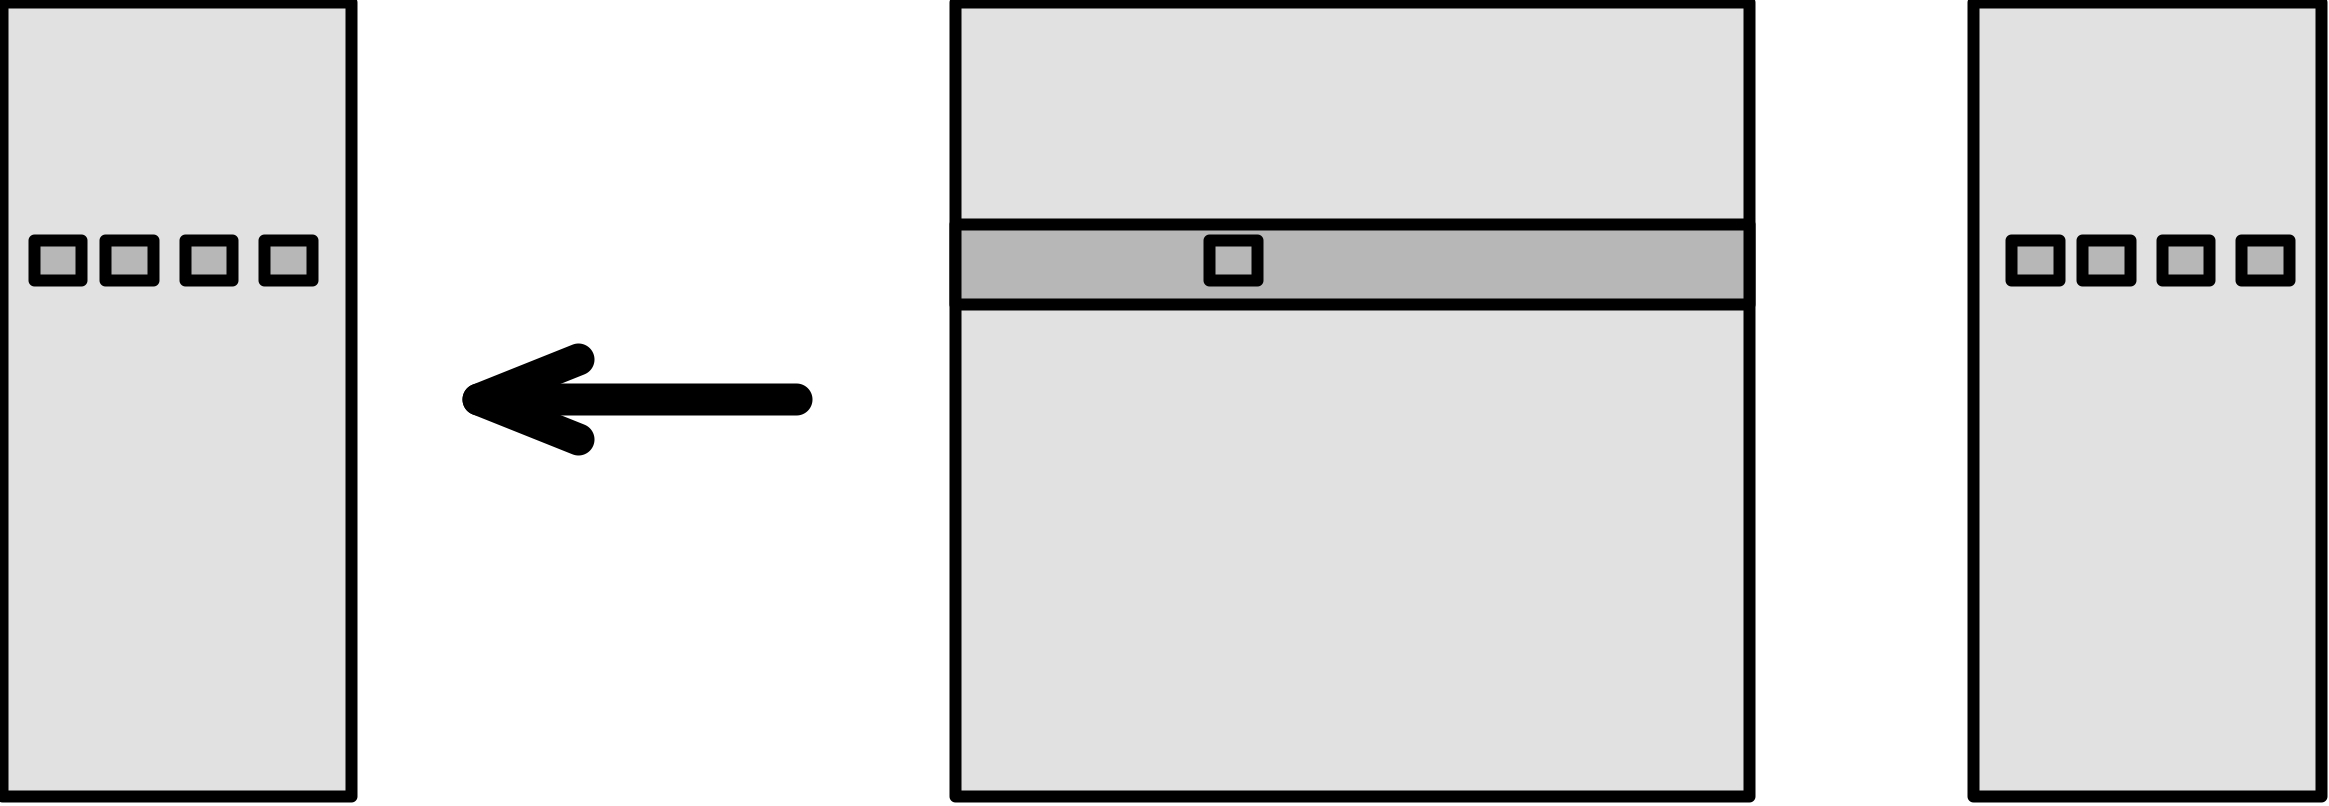
\includegraphics[scale=.12]{gotoblas3}
\caption{The register-resident kernel of the matrix-matrix multiply}
\label{fig:goto3}
\end{figure}
Now this algorithm is tuned.
\begin{itemize}
\item We need enough registers for \verb+C[i,*]+, \verb+A[i,k]+ and
  \verb+B[k,*]+. On current processors that means that we accumulate
  four elements of~$C$.
\item Those elements of~$C$ are accumulated, so they stay in register
  and the only data transfer is loading of the elements of $A$
  and~$B$; there are no stores!
\item The elements \verb+A[i,k]+ and \verb+B[k,*]+ stream from L1.
\item Since the same block of~$A$ is used for many successive slivers
  of~$B$, we want it to stay resident; we choose the blocksize of $A$
  to let it stay in L2 cache.
\item In order to prevent TLB problems, $A$~is stored by rows. If we
  start out with a matrix in (Fortran) \indexterm{column-major}
  storage, this means we have to make a copy. Since copying is of a
  lower order of complexity, this cost is amortizable.
\end{itemize}

\index{matrix-matrix product!Goto implementation|)}

\begin{comment}
\begin{verbatim}
int l1size,l2size, i1,i2, n1,n2;
double *data; int savedptr, ptr = 0;

save2 = 0;
for (i2=0; i2<n2; i2++) {
  save1 = save2;
  for (i1=0; i1<n1; i1++) {
    ptr = save1;
    for ( ; ptr<save1+l1size; ) {
      ..... = .... data[ptr++] ....
    }
    if (i1%3==1) save1 += l1size;
  }
  if (i2%2==1) save2 += l2size;
}
\end{verbatim}
\end{comment}

\endinput
\Level 1 {Arrays and programming languages}

In section~\ref{sec:CFarrays} you can find a discussion of the different
ways arrays are stored in C/C++ and Fortran. These storage modes have
some ramifications on performance. Both from a point of cache line
usage (section~\ref{sec:coding-cacheline}) and prevention of TLB
misses (section~\ref{sec:coding-tlb}) it is best to traverse a
multi-dimensional array so as to access sequential memory locations,
rather than strided. This means that
\begin{itemize}
\item In Fortran you want to loop through an array first by columns
  (that is, in the inner loop),
  then by rows (in the outer loop);
\item In C/C++ you want to loop first through rows (inner loop), then
  through columns (outer loop).
\end{itemize}
